\documentclass[svgnames]{beamer}
\mode<presentation>
\usefonttheme{serif}
\usecolortheme{dove}
\useinnertheme{rounded}
\setbeamercolor{item projected}{fg=black}
\setbeamertemplate{navigation symbols}{}

\usepackage[english]{babel}
\usepackage[latin1]{inputenc}
\usepackage{times}
\usepackage{amsmath}
\usepackage{amsfonts}
\usepackage{amssymb}
\usepackage{amsthm}
\usepackage{graphicx}
\usepackage{multicol}
\usepackage{framed}
\usepackage{ulem}
\usepackage{ifthen}
\usepackage{tikz}
\usepackage{gastex}
\usepackage{ulem}
\usepackage{booktabs}

\newcommand{\set}[1]{\{ #1 \}}
\newcommand{\seq}[1]{\langle #1 \rangle}
\renewcommand{\P}{\mathcal{P}}
\newcommand{\FM}{\mathrm{FM}}
\newcommand{\SAT}{\mathrm{SAT}}
\newcommand{\crochet}[1]{\llbracket #1 \rrbracket}
\newcommand{\crochetc}[1]{\crochet{#1}^\textrm{c}}
\newcommand{\tree}{\mathrm{Tree}}

\newcommand{\At}{\mathbb{A}}
\newcommand{\Orb}{\mathcal{O}}
\newcommand{\A}{\mathcal{A}}
\newcommand{\Pred}{\mathcal{P}}
\newcommand{\N}{\mathbb{N}}
\newcommand{\Z}{\mathbb{Z}}
\newcommand{\Q}{\mathbb{Q}}
\newcommand{\D}{\mathbb{D}}
\newcommand{\M}{\mathcal{M}}
\newcommand{\FO}{\mathrm{FO}}
\newcommand{\NP}{\mathrm{NP}}
\newcommand{\co}{\mathrm{co}}
\newcommand{\PTIME}{\mathrm{PTIME}}
\newcommand{\EXPTIME}{\mathrm{EXPTIME}}
\newcommand{\MSO}{\mathrm{MSO}}
\newcommand{\Atoms}{\mathrm{Atoms}}
\newcommand{\Sym}{\mathrm{Sym}}
\newcommand{\sheet}{\mathrm{Sc}}
\newcommand{\col}{\mathrm{Color}}
\newcommand{\mem}{\mathrm{mem}}
\newcommand{\dom}{\mathrm{dom}}
\newcommand{\orb}{\mathrm{orb}}
\newcommand{\arity}{\mathrm{ar}}

\renewcommand{\ULthickness}{2pt}

%%%%%%%%%%%%%%%%%%%%%%%%%%%%%%%%%%%%%%%%%%%%%%%%%%%%%%%%%%%%%%%%%%%%%%%%%%%%%%%
%%%%%%%%%%%%%%%%%%%% A non-original creation by Nathana�l Fijalkow and myself %

\setbeamertemplate{frametitle}{%
  \vskip-2pt%
  \begin{beamercolorbox}[rightskip=2cm,leftskip=1em,dp=1ex,wd=12.8cm]{frametitle}%
    \vskip2pt%
    \usebeamercolor{frametitle}%
    \begin{tikzpicture}[scale=1]%
      \useasboundingbox (0,0) rectangle (0,0); %(-1,-1) rectangle (1,1);%
      \ifthenelse{\insertframenumber<\inserttotalframenumber}%
      { % uncomplete tart

        \pgfmathsetmacro{\aimangle}{90-(\insertframenumber*360/\inserttotalframenumber)}
        \fill [fill=frametitle.fg,thin, color=gray!50,draw=black] (11.8,.2) -- (11.8,.6) arc (90:\aimangle:0.4) -- cycle;%

      }{ % the full tart
        \fill[fill=frametitle.fg,thin, color=gray!50,draw=black] (11.8,0.2) circle (.4);%
      }%
      \fill[fill=frametitle.fg,thin, color=white,draw=black] (11.8,0.2) circle (.3);%
      \node at (11.8, .2) [black,circle]{\normalsize\insertframenumber};

    \end{tikzpicture}
    \insertframetitle%
    \vskip2pt%
  \end{beamercolorbox}%
}
%%%%%%%%%%%%%%%%%%%%%%%%%%%%%%%%%%%%%%%%%%%%%%%%%%%%%%%%%%%%%%%%%%%%%%%%%%%%%%%


\setbeamertemplate{blocks}[rounded]%
%[shadow=true]
\setbeamercolor{block title}{bg=normal text.bg!90!black}
\setbeamercolor{block body}{bg=normal text.bg!95!black}

\begin{document}

\addtocounter{framenumber}{-1}

\title{Cost-parity games \only<1>{ and Cost-Streett games} \only<2>{\sout{and Cost-Streett games}}}
\subtitle{FSTTCS'2012}
\author{\underline{Nathana\"el Fijalkow}, Martin Zimmermann}
\institute{Institute of Informatics, Warsaw University -- Poland 
\and LIAFA, Universit\'e Paris 7 Denis Diderot -- France}
\date{December 15th, 2012}

\begin{frame}
\maketitle
\end{frame}

\begin{frame}{Framework}

This paper is about two-player games over finite graphs,\\
as used in automata theory and verification (synthesis problem).

\vspace*{3em}

We are after efficient algorithms to:
\begin{itemize}
	\item decide the winner, \textit{and}
	\item synthesize a winning strategy.
\end{itemize}
\vspace*{2em}

\pause
\textit{Starting point:} good understanding of $\omega$-regular specifications.
\vspace*{2em}

\textit{Objective:} add boundedness specifications.

\end{frame}

\begin{frame}{Games}

\begin{multicols}{2}
\begin{picture}(40,60)(0,0)
	\gasset{Nw=8,Nh=8}
	
  	\rpnode[polyangle=45](1)(30,15)(4,5){}
  	\node(2)(20,30){}
  	\node(3)(40,30){}
  	\rpnode[Nmarks=i,iangle=180,polyangle=45](4)(0,30)(4,5){}
  	\rpnode[polyangle=45](5)(10,50)(4,5){}
  	\node(6)(10,10){}
  	\rpnode[polyangle=45](7)(30,50)(4,5){}

  	\drawedge(1,2){}
  	\drawedge[curvedepth=3](1,3){}
	\drawloop[loopangle=90](2){}
  	\drawedge(2,3){}
  	\drawedge(2,6){}
  	\drawedge[curvedepth=5](3,1){}
  	\drawedge(4,2){}
  	\drawedge[curvedepth=5](4,5){}
  	\drawedge[curvedepth=5](5,4){}
	\drawloop[loopangle=-90](6){}
  	\drawedge(7,5){}

\only<3>{\drawedge[AHLength=3,AHlength=4,linecolor=red,linewidth=0.7](4,2){}}
\only<5>{\drawedge[AHLength=3,AHlength=4,linecolor=red,linewidth=0.7](2,6){}}

\only<2,3>{\node[fillcolor=magenta,Nw=4,Nh=4](pebble)(0,30){}} %pebble on 4
\only<4,5>{\node[fillcolor=magenta,Nw=4,Nh=4](pebble)(20,30){}} %pebble on 2
\only<6>{\node[fillcolor=magenta,Nw=4,Nh=4](pebble)(10,10){}} %pebble on 6
\end{picture}

\begin{picture}(40,60)(0,0)
	\gasset{Nw=8,Nh=8}
	
  	\node(Eve)(10,35){}
	\put(16,34){controlled by Eve}
  	\rpnode[polyangle=45](Adam)(10,25)(4,5){}
	\put(16,24){controlled by Adam}
\end{picture}
\end{multicols}
\end{frame}

\begin{frame}{Parity conditions}

\begin{multicols}{2}
\begin{picture}(30,60)(0,0)
	\gasset{Nw=8,Nh=8}

  	\rpnode[polyangle=45](1)(30,15)(4,5){{\color{red}{$1$}}}
  	\node(2)(20,30){{\color{blue}{$2$}}}
  	\node(3)(40,30){{\color{red}{$3$}}}
  	\rpnode[Nmarks=i,iangle=180,polyangle=45](4)(0,30)(4,5){{\color{red}{$3$}}}
  	\rpnode[polyangle=45](5)(10,50)(4,5){{\color{blue}{$2$}}}
  	\node(6)(10,10){{\color{blue}{$4$}}}
  	\rpnode[polyangle=45](7)(30,50)(4,5){{\color{blue}{$0$}}}

  	\drawedge(1,2){}
  	\drawedge[curvedepth=3](1,3){}
	\drawloop[loopangle=90](2){}
  	\drawedge(2,3){}
  	\drawedge(2,6){}
  	\drawedge[curvedepth=5](3,1){}
  	\drawedge(4,2){}
  	\drawedge[curvedepth=5](4,5){}
  	\drawedge[curvedepth=5](5,4){}
	\drawloop[loopangle=-90](6){}
  	\drawedge(7,5){}
\end{picture}

\only<1>{
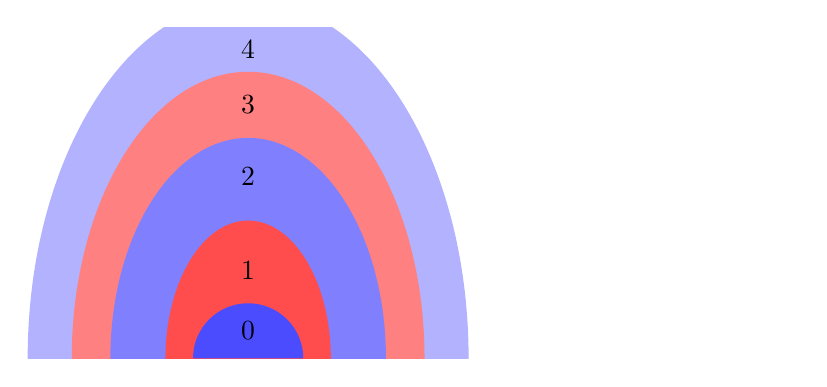
\begin{tikzpicture}[scale=.7]
\clip (-4,0) rectangle (10,6);

% color 4
\fill[white!70!blue] (0,0) ellipse (4cm and 6.5cm) ;
\draw (0,5.6) node {$4$} ;

% color 3
\fill[white!50!red] (0,0) ellipse (3.2cm and 5.2cm) ;
\draw (0,4.6) node {$3$} ;

% color 2
\fill[white!50!blue] (0,0) ellipse (2.5cm and 4cm) ;
\draw (0,3.3) node {$2$} ;

% color 1
\fill[white!30!red] (0,0) ellipse (1.5cm and 2.5cm) ;
\draw (0,1.6) node {$1$} ;

% color 0
\fill[white!30!blue] (-1,0) arc (180:0:1) ;
\node at (0,.5) {$0$};
\end{tikzpicture}
\qquad {\color{red}{Requests}} \quad \qquad {\color{blue}{Responses}}

\begin{framed}
Almost all requests are answered.
\end{framed}
	}

\only<2>{
\vspace*{.7cm}
\begin{itemize}
	\item Parity conditions allow to express all $\omega$-regular specifications.
	\item Both players have positional winning strategies.
	\item Deciding the winner is in $\NP \cap \co\NP$.
\end{itemize}
\vspace*{10cm}
	}
\end{multicols}

\end{frame}

\begin{frame}{Parity and finitary parity}

\only<1>{
Finitary specifications: proposed by Alur and Henzinger,\\
games studied
by Chatterjee, Henzinger and Horn.
}

\begin{multicols}{2}
\begin{framed}
\textbf{Parity:}\\
Almost all requests are answered.
\end{framed}
	
\begin{framed}
\textbf{Finitary parity:}\\
There exists a bound $b$, s.t.\\
almost all requests are answered \textit{within $b$ steps}.
\end{framed}
\vspace*{10em}
\end{multicols}

\only<2>{
\begin{center}
\begin{picture}(40,15)(0,0)
	\gasset{Nw=8,Nh=8}

  	\node(1)(0,5){{\color{red}{$1$}}}
  	\rpnode[polyangle=45](2)(20,10)(4,5){{\color{blue}{$2$}}}
  	\node(0)(40,5){{\color{blue}{$0$}}}

  	\drawedge(1,2){}
	\drawloop[loopangle=90](2){}
  	\drawedge(2,0){}
  	\drawedge[curvedepth=5](0,1){}
\end{picture}
\end{center}
Eve wins for the parity condition, 
\begin{flushright}
but loses for the finitary parity condition!
\end{flushright}
	}

\only<3>{
\begin{multicols}{2}
\begin{itemize}
	\item Both players have positional winning strategies.
	\item Deciding the winner is in $\NP \cap \co\NP$.
\end{itemize}
\vspace*{1em}

\begin{itemize}
	\item Eve has positional winning strategies.
	\item Adam needs infinite memory.
	\item Deciding the winner is in $\PTIME$.
\end{itemize}
\vspace*{3em}
\end{multicols}
	}

\end{frame}


\begin{frame}{Cost-parity games}

\only<1>{
\begin{center}
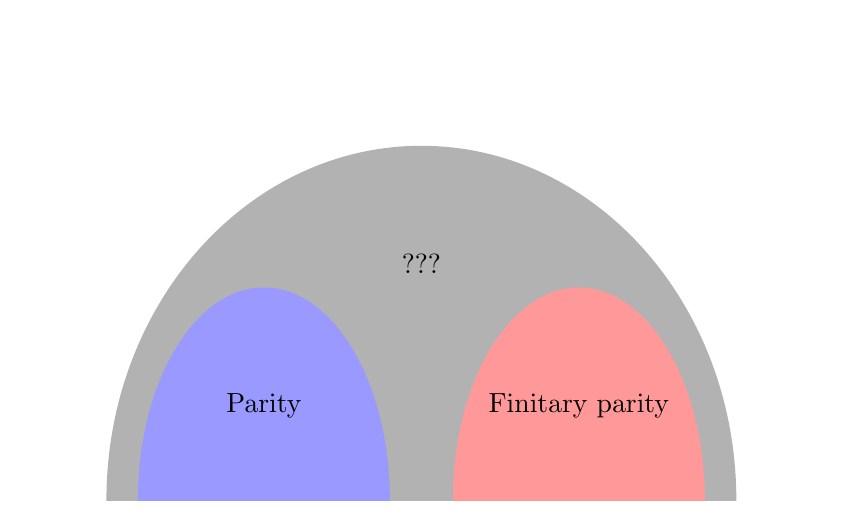
\begin{tikzpicture}
\clip (-5,0) rectangle (5,6);

\fill[white!70!black] (0,0) ellipse (4cm and 4.5cm) ;
\fill[white!60!blue] (-2,0) ellipse (1.6cm and 2.7cm) ;
\fill[white!60!red] (2,0) ellipse (1.6cm and 2.7cm) ;

\draw (-2,1.2) node {Parity} ;
\draw (2,1.2) node {Finitary parity} ;
\draw (0,3) node {???} ;
\end{tikzpicture}
\end{center}
	}

\pause
\begin{center}
\begin{multicols}{2}
\begin{framed}
\textbf{Parity:}\\
Almost all requests are answered.
\end{framed}

\begin{framed}
\textbf{Finitary parity:}\\
There exists a bound $b$, s.t.\\
almost all requests are answered \textit{within $b$ steps}.
\end{framed}
\end{multicols}

\pause

\begin{framed}
\textbf{Cost-parity:}\\
There exists a bound $b$, s.t.\\
almost all requests are answered \textit{with cost at most $b$}.
\end{framed}
\end{center}

\end{frame}

\begin{frame}{Costs}

\begin{center}
\begin{picture}(80,45)(0,0)
	\gasset{Nw=6,Nh=6}

  	\node(1)(0,40){{\color{red}{$1$}}}
  	\rpnode[polyangle=45](2)(15,45)(4,5){{\color{blue}{$2$}}}
  	\node(0)(30,40){{\color{blue}{$0$}}}
	\put(5,27){Parity game}

  	\drawedge(1,2){$\varepsilon$}
	\drawloop[loopangle=90](2){$\varepsilon$}
  	\drawedge(2,0){$\varepsilon$}
  	\drawedge[curvedepth=5](0,1){$\varepsilon$}

  	\node(1b)(50,40){{\color{red}{$1$}}}
  	\rpnode[polyangle=45](2b)(65,45)(4,5){{\color{blue}{$2$}}}
  	\node(0b)(80,40){{\color{blue}{$0$}}}
	\put(50,27){Finitary parity game}

  	\drawedge(1b,2b){i}
	\drawloop[loopangle=90](2b){i}
  	\drawedge(2b,0b){i}
  	\drawedge[curvedepth=5](0b,1b){i}

  	\node(1bb)(25,0){{\color{red}{$1$}}}
  	\rpnode[polyangle=45](2bb)(40,5)(4,5){{\color{blue}{$2$}}}
  	\node(0bb)(55,0){{\color{blue}{$0$}}}

  	\drawedge(1bb,2bb){i}
	\drawloop[loopangle=90](2bb){$\varepsilon$}
  	\drawedge(2bb,0bb){i}
  	\drawedge[curvedepth=5](0bb,1bb){$\varepsilon$}
\end{picture}
\end{center}

\end{frame}

\begin{frame}{Positional determinacy for Eve}
Objective: \textbf{strategy optimization}\\
\begin{framed}
Assume $\sigma$ is a winning strategy.\\
How to construct a memoryless winning strategy $\sigma'$ from $\sigma$?
\end{framed}
\pause
Tool: \textbf{scoring functions}
\vskip2em
``\`a la M\"uller and Schupp'' past-oriented proof
\end{frame}

\begin{frame}{A general framework}
Consider a winning strategy $\sigma : V^* \rightarrow V$.
\vskip1em
Define a scoring function $\sheet : V^* \rightarrow (S,\le)$ satisfying:
\pause
\begin{enumerate}
	\item $(S,\le)$ is a total order and $\sheet$ is a congruence:\\
	if $\sheet(w) \le \sheet(w')$, 
	then $\sheet(w \cdot v) \le \sheet(w' \cdot v)$.
% \item The score-sheets are totally ordered.
% \item The score-sheet function is a congruence w.r.t.\ this order.
\vskip1em
\pause
	\item If there exists a bound~$b$ such that the scores of all prefixes of a play~$\rho$ are bounded
	by $b$, then $\rho$ is winning.
% \item If the score-sheets of a play are bounded, then it is winning for Player~$0$.
\vskip1em
\pause
	\item Assume a play $\rho$ is consistent with $\sigma$, 
	then the scores of all prefixes of $\rho$ are (uniformly) bounded.
%	A finite-state winning strategy uniformly bounds the score-sheets of all plays.
\end{enumerate}
\pause
\vskip1em
Construct a memoryless strategy $\sigma'$: 
\begin{center}
``play according to $\sigma$ assuming the worst play prefix''.
\end{center}
\end{frame}

\begin{frame}{Deciding the winner in cost-parity games}
$n$: number of vertices\\
$m$: number of edges\\
$d$: number of colors
\vskip2em
\begin{theorem}
Given a parity games solver of complexity $T(n,m,d)$,\\
there exists a cost-parity games solver of complexity 
$$O(n \cdot T(n \cdot d,m \cdot d,d+2))\ .$$
\end{theorem}
\end{frame}

\begin{frame}{Results}
$$\begin{array}{llll}
\toprule
\textrm{winning condition} & \textrm{complexity} & \textrm{Eve} & \textrm{Adam} \\
\midrule
\textrm{parity} & {\color{red}{\NP \cap \co\NP}} & {\color{red}{\textrm{memoryless}}} & \textrm{memoryless} \\
\textrm{finitary parity} & \PTIME & {\color{red}{\textrm{memoryless}}} & {\color{red}{\textrm{infinite}}} \\
\textrm{cost-parity} & \NP \cap \co\NP & \textrm{memoryless} & \textrm{infinite} \\
\midrule
\textrm{Streett} & \co\NP\textrm{-complete} & {\color{red}{\textrm{finite}}} & \textrm{memoryless} \\
\textrm{finitary Streett} & {\color{red}{\EXPTIME\textrm{-complete}}} & {\color{red}{\textrm{finite}}} & {\color{red}{\textrm{infinite}}} \\
\textrm{cost-Streett} & \EXPTIME\textrm{-complete} & \textrm{finite} & \textrm{infinite} \\
\bottomrule
\end{array}$$
\end{frame}

\begin{frame}{Towards $\omega$B-conditions}
\begin{center}
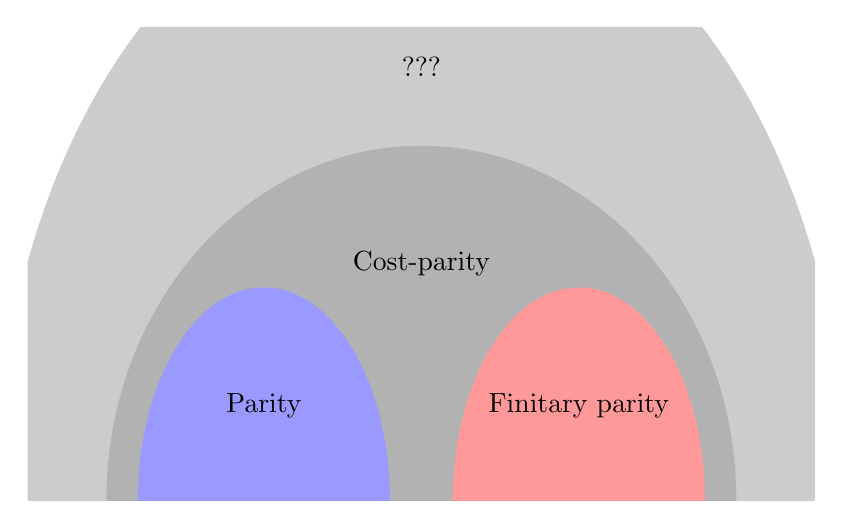
\begin{tikzpicture}
\clip (-5,0) rectangle (5,6);

\fill[white!80!black] (0,0) ellipse (5.4cm and 8cm) ;
\fill[white!70!black] (0,0) ellipse (4cm and 4.5cm) ;
\fill[white!60!blue] (-2,0) ellipse (1.6cm and 2.7cm) ;
\fill[white!60!red] (2,0) ellipse (1.6cm and 2.7cm) ;

\draw (-2,1.2) node {Parity} ;
\draw (2,1.2) node {Finitary parity} ;
\draw (0,3) node {Cost-parity} ;
\draw (0,5.5) node {???} ;
\end{tikzpicture}
\end{center}
\end{frame}



\end{document}